%\documentclass[authoryear,5p]{elsarticle}
\documentclass[authoryear,preprint,11pt]{elsarticle}
\bibliographystyle{elsarticle-harv}
\usepackage{graphicx}
\usepackage{amsmath,amsfonts}
\usepackage{lineno}
\linenumbers
\usepackage{subfigure}
\usepackage[pdftex]{color}
\definecolor{darkblue}{rgb}{0,0,0.5}
\definecolor{darkgreen}{rgb}{0,0.5,0}
%\usepackage[pdftex, colorlinks, citecolor=darkblue,linkcolor=darkgreen]{hyperref}
\usepackage[pdftex, colorlinks]{hyperref}
\textwidth 6.75in
\oddsidemargin -0.15in
\evensidemargin -0.15in
\textheight 9in
\topmargin -0.5in
\newcommand{\ud}{\mathrm{d}}
\newcommand{\E}{\mathrm{E}}
\newcommand{\C}{\mathrm{Cov}}
\newcommand{\V}{\mathrm{Var}}

\newcommand{\cb}[1]{{\it \color{darkgreen} (#1)}}



\journal{\tiny } 
\begin{document}
\begin{frontmatter}
  \title{Early Warning Signals and the Prosecutor's Fallacy}
  \author[cpb]{Carl Boettiger\corref{cor1}}
  \ead{cboettig@ucdavis.edu}
  \author[esp]{Alan Hastings}
  %\author[info]{}
  %\author[davis]{}
  \cortext[cor1]{Corresponding author.}
  \address[cpb]{Center for Population Biology, 1 Shields Avenue, University of California, Davis, CA, 95616 United States.}
  \address[esp]{Department of Environmental Science and Policy, University of California, Davis} 

 % \address[info]{ \\ 
  %              }

  \begin{abstract}

  Early warning signals have been proposed to forecast the possibility of a 
  critical transition, such as the eutriphication of a lake, desertification
  of savanna, the collapse of a coral reef, the end of a glacial period, or 
  the onset of epilepsy in the brain.  While such transitions may be difficult
  to study in the laboratory setting and unethical to introduce on the a larger
  natural scales where they may occur, it has often been observed that history
  has already performed the experiment for us, time and again.  Here we point 
  out a critical difference between selecting systems for study based on the 
  fact that we have observed a critical transition and those systems for which
  we wish to forecast the approach of a transition. This difference arising
  from conditional probabilities is often known as the the Prosecutor's 
  Fallacy.  We illustrate through simulation how examples of systems that have 
  experienced transitions purely by chance show patterns associated with 
  early warning signals more often than we might expect in systems that have not
  been conditionally selected.  We further highlight how a model-based approach
  is less subject to this bias.  In using historical examples of collapse to 
  test and validate methods for early warning signals, greater care must be taken
  to avoid this fallacy.
 
  \end{abstract}

  \begin{keyword}
early warning signals \sep tipping point \sep alternative stable states \sep likelihood methods 
   \end{keyword}
 \end{frontmatter}

 \section{Introduction}

 \section{Methods and Results}
 We simulated 1000 replicates of an individual-based birth-death process with an allee threshold.  Above the allee threshold the population returns to a positive equilibrium size.  Below the threshold the population decreases to zero. The simulation uses the Gillespie algorithm to provide an exact implementation of the master equation of birth-death process,

\begin{align}
  \frac{dP(n,t)}{dt} &= b_{n-1} P(n-1,t) + d_{n+1}P(n+1,t) - (b_n+d_n) P(n,t)  \label{master} \\
    b_n &= \frac{e K n^2}{n^2 + h^2} \\
    d_n &= e n + a
\end{align}

Though this system can be forced through a saddle-node bifurcation by
increasing values of either $e$ or $a$, all parameters are held fixed.
The simulation starts from the positive equilibrium population size.
Though the chance of a transition across the allee threshold in any 
given timestep are small, given enough time this system will eventually
experience such a rare event driving the population extinct.  We evolved
each replicate 50000 timesteps, sampling the system every 50 timesteps.  
In this time window 155 of the 1000 replicates experience population collapse.  
Nine of these replicates can be seen in Figure~\ref{fig:replicate_crashes},
as an illustration. 

We selected replicates conditional on having collapsed in the simulations.
We then selected a window around each system that ended just before the
collapse, while the population values were still above the allee threshold.
For each replicate, we calculated the most common warning signals, variance
and autocorrelation~\citep[\emph{e.g.}][]{Carpenter2006,Dakos2008,Scheffer2009}, 
around a moving window equal to half the length of that
timeseries.  

To determine whether or not the variance or autocorrelation increased 
over time in these 155 replicates, we computed Kendall's $\tau$ for each of the
warning signal pattern~\citep{Dakos2008, Dakos2010}.  Positive values of $\tau$ 
indicate an increasing trend in the warning signal.  The distribution of $\tau$ 
values observed across these replicates is shown in Figure~\ref{fig:indicator}.
More positive values indicate stronger trends. Assessing the statistical significance
of a given value requires an appropriate null model, which can be difficult 
to do~\citep{Dakos2008}. As these examples have been selected from a system
that is not approaching a bifurcation and therefore should not exhibit any 
early warning sign, even the very strong values of $\tau$ should be considered 
as arising from the null model. 

We compared this approach to a model-based approach 


  \begin{figure}[ht]
    \begin{center}
      \includegraphics{replicate_crashes}
    \end{center}
    \caption{Nine of the 155 replicates that experience a critical transition by chance during the course of the simulation.}
    \label{fig:replicate_crashes}
  \end{figure}


  \begin{figure}[ht]
    \begin{center}
      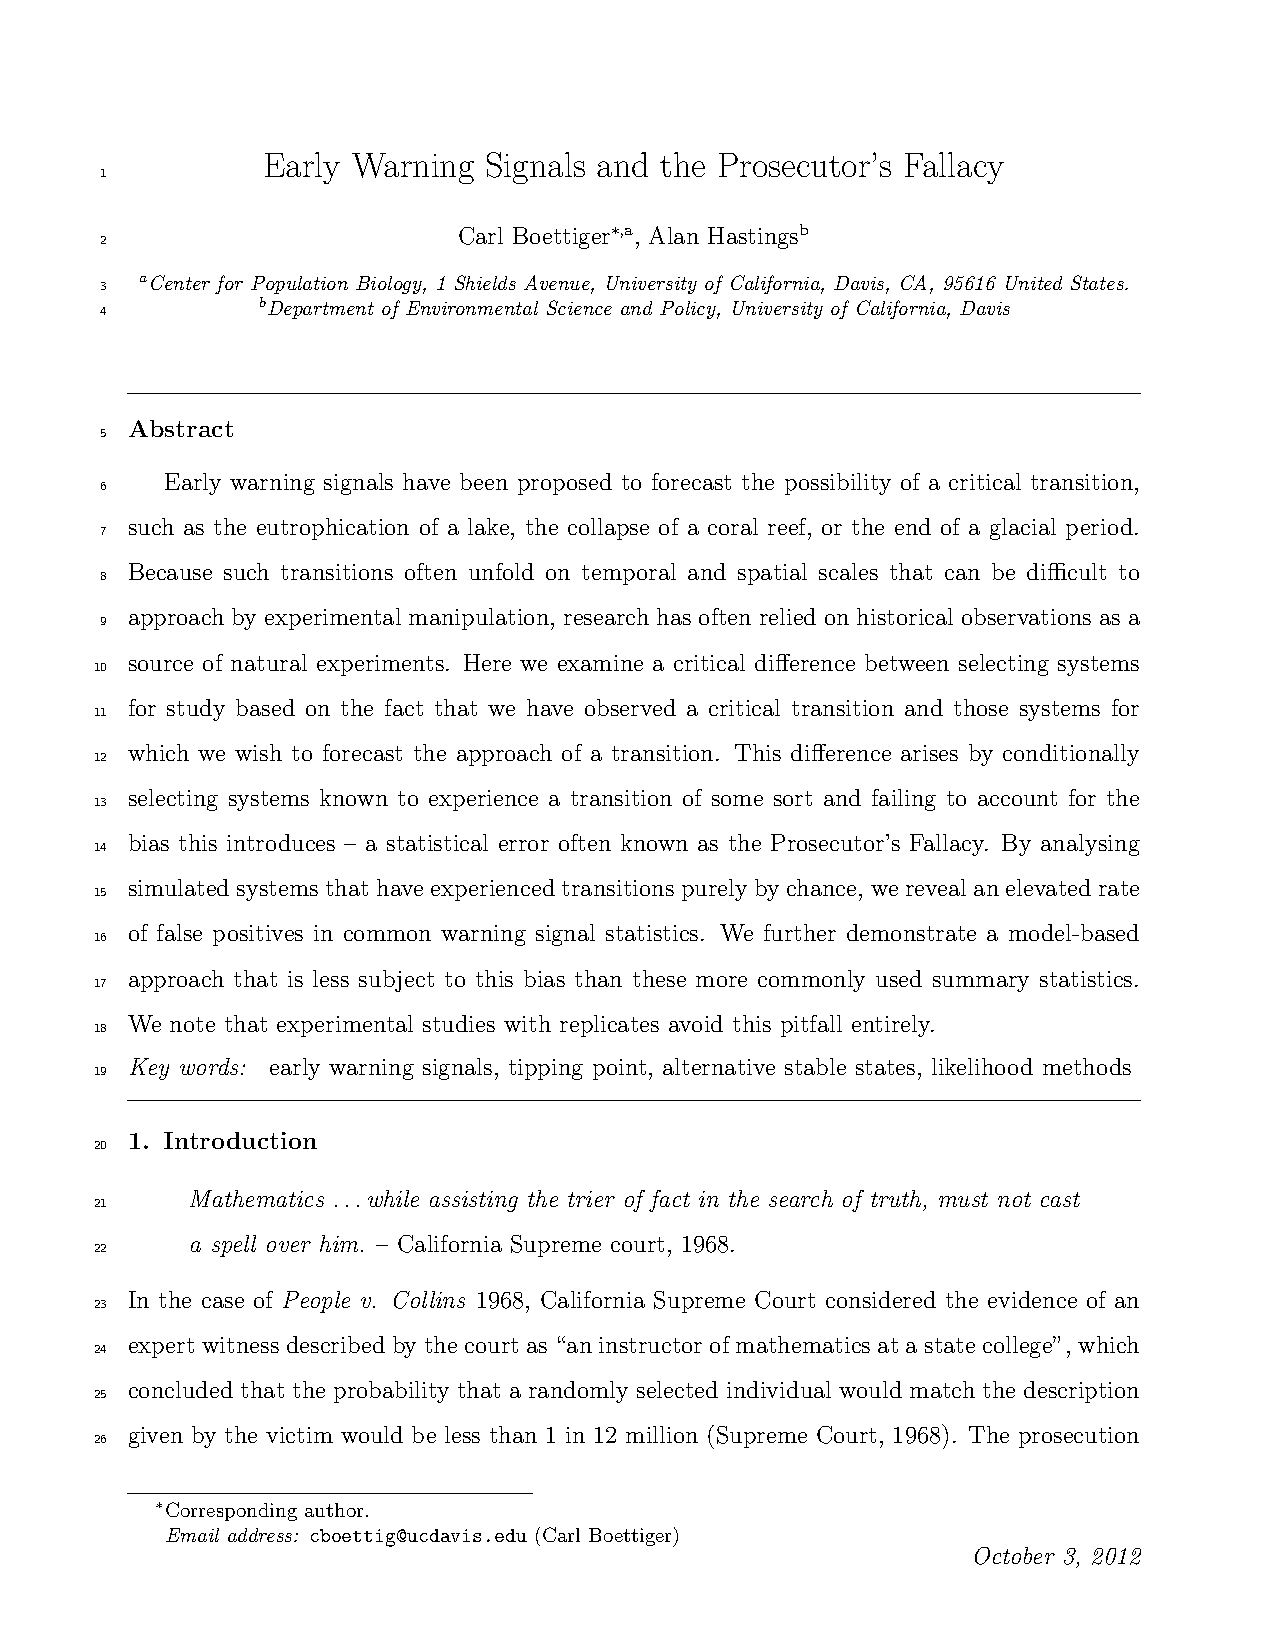
\includegraphics{fallacy}
    \end{center}
    \caption{The distribution of three early warning indicators on replicates conditionally selected for having collapsed by chance in simulations.}
    \label{fig:indicator}
  \end{figure}

 \section{Discussion}

 \section{References}%bibliography
 \bibliography{boettiger}
 \end{document}



